\documentclass[a4paper,twoside,openright,makeidx,12pt]{book}
%\usepackage{draftcopy}
%%$Id: macro.tex,v 1.10 2004/12/08 13:38:58 acary Exp $


%\usepackage{a4wide}
\textheight 25cm
\textwidth 16.5cm
\topmargin -1cm
%\evensidemargin 0cm
\oddsidemargin 0cm
\evensidemargin0cm
\usepackage{layout}


\usepackage{amsmath}
\usepackage{amssymb}
\usepackage{minitoc}
%\usepackage{glosstex}
\usepackage{colortbl}
\usepackage{hhline}
\usepackage{longtable}

%\usepackage{glosstex}
%\def\glossaryname{Glossary of Notation}
\def\listacronymname{Acronyms}

\usepackage[outerbars]{changebar}\setcounter{changebargrey}{20}
%\glxitemorderdefault{acr}{l}

%\usepackage{color}
\usepackage{graphicx,epsfig}
\graphicspath{{figure/}}
\usepackage[T1]{fontenc}
\usepackage{rotating}

%\usepackage{algorithmic}
%\usepackage{algorithm}
\usepackage{ntheorem}
\usepackage{natbib}


%\renewcommand{\baselinestretch}{2.0}
\setcounter{tocdepth}{2}     % Dans la table des matieres
\setcounter{secnumdepth}{3}  % Avec un numero.



\newtheorem{definition}{Definition}
\newtheorem{lemma}{Lemma}
\newtheorem{claim}{Claim}
\newtheorem{remark}{Remark}
\newtheorem{assumption}{Assumption}
\newtheorem{example}{Example}
\newtheorem{conjecture}{Conjecture}
\newtheorem{corollary}{Corollary}
\newtheorem{OP}{OP}
\newtheorem{problem}{Problem}
\newtheorem{theorem}{Theorem}


\newcommand{\CC}{\mbox{\rm $~\vrule height6.6pt width0.5pt depth0.25pt\!\!$C}}
\newcommand{\ZZ}{\mbox{\rm \lower0.3pt\hbox{$\angle\!\!\!$}Z}}
\newcommand{\RR}{\mbox{\rm $I\!\!R$}}
\newcommand{\NN}{\mbox{\rm $I\!\!N$}}

\newcommand{\Mnn}{\mathcal M^{n\times n}}
\newcommand{\Mnp}[2]{\ensuremath{\mathcal M^{#1\times #2}}}



\newcommand{\Frac}[2]{\displaystyle \frac{#1}{#2}}

\newcommand{\DP}[2]{\displaystyle \frac{\partial {#1}}{\partial {#2}}}

% c++ variables writting
\newcommand{\varcpp}[1]{\textit{#1}}
% itemize
\newcommand{\bei}{\begin{itemize}}
\newcommand{\ei}{\end{itemize}}

\newcommand{\ie}{i.e.}
\newcommand{\eg}{e.g.}
\newcommand{\cf}{c.f.}
\newcommand{\putidx}[1]{\index{#1}\textit{#1}}

\def\Er{{\rm I\! R}}
\def\En{{\rm I\! N}} 
\def\Ec{{\rm I\! C}}
 
\def\zc{\hat{z}}
\def\wc{\hat{w}}

\font\tete=cmr8 at 8 pt
\font\titre= cmr12 at 20 pt 
\font\titregras=cmbx12 at 20 pt

%----------------------------------------------------------------------
%                  Modification des subsubsections
%----------------------------------------------------------------------
\makeatletter
\renewcommand\thesubsubsection{\thesubsection.\@alph\c@subsubsection}
\makeatother

%----------------------------------------------------------------------
%             Redaction note environnement
%----------------------------------------------------------------------
\makeatletter
\theoremheaderfont{\scshape}
\theoremstyle{marginbreak}
\theorembodyfont{\upshape}
%\newtheorem{rque}{\bf Remarque}[chapter]
%\newtheorem{rque1}{\bf \fsc{Remarque}}[chapter] !!! \fsc est une commande french
\newtheorem{ndr1}{\textbf{\textsc{Redaction note}}}[section]

\newenvironment{ndr}%
{%
\tt
%\centerline{---oOo---}
\noindent\begin{ndr1}%
}%
{%
\begin{flushright}%
%\vspace{-1.5em}\ding{111}
\end{flushright}%
\end{ndr1}%
%\centerline{---oOo---}
}

\makeatother

%----------------------------------------------------------------------
%             Redaction note environnement V.ACARY
%----------------------------------------------------------------------
\makeatletter
\theoremheaderfont{\scshape}
\theoremstyle{marginbreak}
\theorembodyfont{\upshape}
%\newtheorem{rque}{\bf Remarque}[chapter]
%\newtheorem{rque1}{\bf \fsc{Remarque}}[chapter] !!! \fsc est une commande french
\newtheorem{ndr1va}{\textbf{\textsc{Redaction note V. ACARY}}}[section]

\newenvironment{ndrva}%
{%
\tt
%\centerline{---oOo---}
\noindent\begin{ndr1va}%
}%
{%
\begin{flushright}%
%\vspace{-1.5em}\ding{111}
\end{flushright}%
\end{ndr1va}%
%\centerline{---oOo---}
}

\makeatother
%----------------------------------------------------------------------
%             Redaction note environnement V.ACARY
%----------------------------------------------------------------------
\makeatletter
\theoremheaderfont{\scshape}
\theoremstyle{marginbreak}
\theorembodyfont{\upshape}
%\newtheorem{rque}{\bf Remarque}[chapter]
%\newtheorem{rque1}{\bf \fsc{Remarque}}[chapter] !!! \fsc est une commande french
\newtheorem{ndr1fp}{\textbf{\textsc{Redaction note F. PERIGNON}}}[section]

\newenvironment{ndrfp}%
{%
\tt
%\centerline{---oOo---}
\noindent\begin{ndr1fp}%
}%
{%
\begin{flushright}%
%\vspace{-1.5em}\ding{111}
\end{flushright}%
\end{ndr1fp}%
%\centerline{---oOo---}
}

\makeatother
%----------------------------------------------------------------------
%                  Chapter head enviroment
%----------------------------------------------------------------------
\newenvironment{chapter_head}
{%
\begin{center}%
-------------------- oOo --------------------\\%
\ \\%
\begin{minipage}[]{14cm}%
\noindent\normalsize\advance\baselineskip-1pt %
}%
{%
\par\end{minipage}%
\ \\%
\ \\%
-------------------- oOo --------------------
\end{center}%
\vspace*{\stretch{1}}%
\clearpage%
\thispagestyle{empty}%
\vspace*{\stretch{1}}%
\minitoc%
\vspace*{\stretch{2}}%
\clearpage%
}

%%% Local Variables: 
%%% mode: latex
%%% TeX-master: "report"
%%% End: 

%$Id: macro.tex,v 1.10 2004/12/08 13:38:58 acary Exp $


%\usepackage{a4wide}
\textheight 25cm
\textwidth 16.5cm
\topmargin -1cm
%\evensidemargin 0cm
\oddsidemargin 0cm
\evensidemargin0cm
\usepackage{layout}


\usepackage{amsmath}
\usepackage{amssymb}
\usepackage{minitoc}
%\usepackage{glosstex}
\usepackage{colortbl}
\usepackage{hhline}
\usepackage{longtable}

%\usepackage{glosstex}
%\def\glossaryname{Glossary of Notation}
\def\listacronymname{Acronyms}

\usepackage[outerbars]{changebar}\setcounter{changebargrey}{20}
%\glxitemorderdefault{acr}{l}

%\usepackage{color}
\usepackage{graphicx,epsfig}
\graphicspath{{figure/}}
\usepackage[T1]{fontenc}
\usepackage{rotating}

%\usepackage{algorithmic}
%\usepackage{algorithm}
\usepackage{ntheorem}
\usepackage{natbib}


%\renewcommand{\baselinestretch}{2.0}
\setcounter{tocdepth}{2}     % Dans la table des matieres
\setcounter{secnumdepth}{3}  % Avec un numero.



\newtheorem{definition}{Definition}
\newtheorem{lemma}{Lemma}
\newtheorem{claim}{Claim}
\newtheorem{remark}{Remark}
\newtheorem{assumption}{Assumption}
\newtheorem{example}{Example}
\newtheorem{conjecture}{Conjecture}
\newtheorem{corollary}{Corollary}
\newtheorem{OP}{OP}
\newtheorem{problem}{Problem}
\newtheorem{theorem}{Theorem}


\newcommand{\CC}{\mbox{\rm $~\vrule height6.6pt width0.5pt depth0.25pt\!\!$C}}
\newcommand{\ZZ}{\mbox{\rm \lower0.3pt\hbox{$\angle\!\!\!$}Z}}
\newcommand{\RR}{\mbox{\rm $I\!\!R$}}
\newcommand{\NN}{\mbox{\rm $I\!\!N$}}

\newcommand{\Mnn}{\mathcal M^{n\times n}}
\newcommand{\Mnp}[2]{\ensuremath{\mathcal M^{#1\times #2}}}



\newcommand{\Frac}[2]{\displaystyle \frac{#1}{#2}}

\newcommand{\DP}[2]{\displaystyle \frac{\partial {#1}}{\partial {#2}}}

% c++ variables writting
\newcommand{\varcpp}[1]{\textit{#1}}
% itemize
\newcommand{\bei}{\begin{itemize}}
\newcommand{\ei}{\end{itemize}}

\newcommand{\ie}{i.e.}
\newcommand{\eg}{e.g.}
\newcommand{\cf}{c.f.}
\newcommand{\putidx}[1]{\index{#1}\textit{#1}}

\def\Er{{\rm I\! R}}
\def\En{{\rm I\! N}} 
\def\Ec{{\rm I\! C}}
 
\def\zc{\hat{z}}
\def\wc{\hat{w}}

\font\tete=cmr8 at 8 pt
\font\titre= cmr12 at 20 pt 
\font\titregras=cmbx12 at 20 pt

%----------------------------------------------------------------------
%                  Modification des subsubsections
%----------------------------------------------------------------------
\makeatletter
\renewcommand\thesubsubsection{\thesubsection.\@alph\c@subsubsection}
\makeatother

%----------------------------------------------------------------------
%             Redaction note environnement
%----------------------------------------------------------------------
\makeatletter
\theoremheaderfont{\scshape}
\theoremstyle{marginbreak}
\theorembodyfont{\upshape}
%\newtheorem{rque}{\bf Remarque}[chapter]
%\newtheorem{rque1}{\bf \fsc{Remarque}}[chapter] !!! \fsc est une commande french
\newtheorem{ndr1}{\textbf{\textsc{Redaction note}}}[section]

\newenvironment{ndr}%
{%
\tt
%\centerline{---oOo---}
\noindent\begin{ndr1}%
}%
{%
\begin{flushright}%
%\vspace{-1.5em}\ding{111}
\end{flushright}%
\end{ndr1}%
%\centerline{---oOo---}
}

\makeatother

%----------------------------------------------------------------------
%             Redaction note environnement V.ACARY
%----------------------------------------------------------------------
\makeatletter
\theoremheaderfont{\scshape}
\theoremstyle{marginbreak}
\theorembodyfont{\upshape}
%\newtheorem{rque}{\bf Remarque}[chapter]
%\newtheorem{rque1}{\bf \fsc{Remarque}}[chapter] !!! \fsc est une commande french
\newtheorem{ndr1va}{\textbf{\textsc{Redaction note V. ACARY}}}[section]

\newenvironment{ndrva}%
{%
\tt
%\centerline{---oOo---}
\noindent\begin{ndr1va}%
}%
{%
\begin{flushright}%
%\vspace{-1.5em}\ding{111}
\end{flushright}%
\end{ndr1va}%
%\centerline{---oOo---}
}

\makeatother
%----------------------------------------------------------------------
%             Redaction note environnement V.ACARY
%----------------------------------------------------------------------
\makeatletter
\theoremheaderfont{\scshape}
\theoremstyle{marginbreak}
\theorembodyfont{\upshape}
%\newtheorem{rque}{\bf Remarque}[chapter]
%\newtheorem{rque1}{\bf \fsc{Remarque}}[chapter] !!! \fsc est une commande french
\newtheorem{ndr1fp}{\textbf{\textsc{Redaction note F. PERIGNON}}}[section]

\newenvironment{ndrfp}%
{%
\tt
%\centerline{---oOo---}
\noindent\begin{ndr1fp}%
}%
{%
\begin{flushright}%
%\vspace{-1.5em}\ding{111}
\end{flushright}%
\end{ndr1fp}%
%\centerline{---oOo---}
}

\makeatother
%----------------------------------------------------------------------
%                  Chapter head enviroment
%----------------------------------------------------------------------
\newenvironment{chapter_head}
{%
\begin{center}%
-------------------- oOo --------------------\\%
\ \\%
\begin{minipage}[]{14cm}%
\noindent\normalsize\advance\baselineskip-1pt %
}%
{%
\par\end{minipage}%
\ \\%
\ \\%
-------------------- oOo --------------------
\end{center}%
\vspace*{\stretch{1}}%
\clearpage%
\thispagestyle{empty}%
\vspace*{\stretch{1}}%
\minitoc%
\vspace*{\stretch{2}}%
\clearpage%
}

%%% Local Variables: 
%%% mode: latex
%%% TeX-master: "report"
%%% End: 

\usepackage{pifont}
 \usepackage{lscape}



\includeonly{}
\usepackage{fancyheadings} 
\usepackage{verbatim}

% package pour les images des use cases
%\usepackage[dvips]{graphicx}

\pagestyle{fancy} 
\renewcommand{\chaptermark}[1]% 
{\markboth{{Chap-- \thechapter.\ #1}}{}} 
\renewcommand{\sectionmark}[1]% 
{\markright{{\thesection.\ #1}}} 
\setlength{\headrulewidth}{0.5pt} 
\setlength{\footrulewidth}{0.5pt} 
\newcommand{\helv}{% 
\fontfamily{phv}\fontseries{b}\fontsize{9}{11}\selectfont} 
\lhead[\helv \thepage]{\helv \rightmark} 
\rhead[\helv \leftmark]{\helv \thepage} 
\cfoot{Software Specification Document -- November 25, 2004}

\makeindex

\begin{document}
\pagestyle{empty}
\renewcommand{\arraystretch}{1.8}

%%%%%%%%%%%%%%%%%%%%%%%%%%%%%%%%%%%%%%%%%%%%%%%%%%%%%%%%%%%%%%%%%%%%%%%%%%%%%%%%%%%%%%%%%%%%%%%%%%%%%%%%%
%\documentclass[titlepage, 12pt]{report}

%\usepackage[dvips]{graphicx}
%\usepackage{graphics}
%\usepackage{amssymb}
%\usepackage{latexsym}


%\begin{document}

\thispagestyle{empty}

\begin{center}

\includegraphics[height=23mm, width=77mm]{figure/siconos.eps}\\
\textsf{European Project IST2001-37172}\\[6cm]
\end{center}

\begin{center}
\huge
\textsf{\textbf{\textit{Software Specification Document}}}\\[2.5cm]
\end{center}

\large
\begin{center}
\textsf{\textbf{Version :} 0.1}\\
\textsf{\textbf{Status :}  In progress}\\
\textsf{\textbf{Date : } December 17, 2004}\\
\textsf{\textbf{Document Code :} NUMERICS/SSD}\\[5cm]

\end{center}

\normalsize

\begin{flushright}

\includegraphics[scale=0.3]{figure/Logo-INRIA.eps}
\end{flushright}

\clearpage




%\maketitle

%-----------------------------------------------------------------------------%

\normalsize

\begin{center}
  \textsf{\Large Identification}
\end{center}

\noindent\begin{tabular}{|p{0.3\textwidth}|p{0.7\textwidth}|}
\hline
Document Title : & \textsf{Software Specification Document} \\
Document Code :  & \textsf{NUMERICS/SSD} \\
\hline
\end{tabular}
\textsf{ }\\


\begin{center}
  \textsf{\Large About the document and its author(s)}
\end{center}

\noindent\begin{tabular}{|p{0.3\textwidth}|p{0.7\textwidth}|}
\hline
Nature :& \textsf{This document defines the Software Specification for Numerics}\\
Language :& \textsf{English}\\
Author(s) :& \textsf{Vincent ACARY, Fr�d�ric DUBOIS, Jean-Michel BARBIER}\\
\hline
\end{tabular}

\textsf{ }\\

%\newpage

% cartridge current version
\begin{center}
  \textsf{\Large Current Version}
\end{center}
\begin{tabular}{|p{0.3\textwidth}|p{0.7\textwidth}|}
\hline
Date : &\textsf{December 17, 2004}\\
Current version number : &\textsf{0.1}\\ 
Status :&$\bigotimes$ in progress \\
& $\bigcirc$ validated\\
\textit{ }& \hspace{0.5cm} Approved by :\\
\hline
Document change record since last version : &
\begin{minipage}[t]{0.70\textwidth}
  \begin{itemize}
  \item \textsf{Architecture design in progress} \\
  \end{itemize}
\end{minipage}\\
\hline
\end{tabular}


\textsf{ }\\
\begin{center}
\textbf{Copyright Notice \copyright}\\
This document may not be reproduced (even partially) or communicated to third parties without the written authorisation of LMGC.
\end{center}


% log of changes  
\pagebreak
\begin{center}
  \textsf{\Large About the document developing process}
\end{center}
\begin{tabular}{|p{0.3\textwidth}|p{0.7\textwidth}|}
\hline
Date of first issue : &\textsf{November 25, 2004}\\
Current version number : &\textsf{0.1}\\ 
Validated by :& \textsf{}\\
\hline
Document change record since last version : &\textsf{First issue} \\
\hline

\end{tabular}

%\end{document}

%%%%%%%%%%%%%%%%%%%%%%%%%%%%%%%%%%%%%%%%%%%%%%%%%%%%%%%%%%%%%%%%%%%%%%%%%%%%%%%%%%%%%%%%%%%%%%%%%%%%%%%%%


\tableofcontents


\pagestyle{fancy}
%---------------------------------------------------------------------%
\cleardoublepage

\pagenumbering{arabic}
\chapter{Introduction}
\label{Sec:SSD-Intoduction}
\section{Purpose of this document}
\label{Sec:SUM-Purpose-Scope}
The purpose of the Software User Manual is to ...



%---------------------------------------------------------------------%
\newpage
\chapter{Specific requirements}
\label{Sec:SSD-SpecificRequirements}
%---------------------------------------------------------------------------%
\section{Model and numerical methods related requirements}

%---------------------------------------------------------------------------%
\section{Functional requirements}
\label{Sec:SRD-FunctionalRequirements}
%\subsection{\ac{siconos}/Numerics}
\begin{longtable}{%
    |>{\columncolor[gray]{.8}}p{0.1\textwidth}%
    |>{\columncolor[gray]{.95}}p{0.9\textwidth}|}
  \hline
  \rowcolor[gray]{.8}   SR. Id. & Software requirements description \\
  \hline 
  \hline
  & \textbf{General  requirements (\ac{siconos}/Numerics)}\\
  \hline 
  F.1.001 & The module \ac{siconos}/Numerics must provide basic algebra objects (vector, matrices, quaternions) \bf{ \sf relying on a matrix template library} \\
  F.1.002 & The module \ac{siconos}/Numerics must provide  high performance methods for  basic vector and matrix operations\\
  F.1.003 & The module \ac{siconos}/Numerics must support various storage methods for matrices:
  \begin{enumerate}
  \item Dense(full)
  \item Band
%fd sans interet  \item Skyline
  \item Sparse
  \end{enumerate}\\
 \hline 
 & \textbf{ Numerical functionalities  requirements (\ac{siconos}/Numerics)}\\
  \hline
  F.1.010 & The module  \ac{siconos}/Numerics has to perform basic linear algebra computations  relying on standard libraries for numerical computation (e.g. LAPACK):
  \begin{enumerate}
  \item Solution of linear system 
  \item Eigenvalue and eigenvectors problem
  \item Singular Value Decomposition
  \end{enumerate}
  \\
  F.1.011 & The module \ac{siconos}/Numerics has to perform solution for mathematical programming problems:
  \begin{enumerate}
  \item Linear Complementarity Problem (LCP) (direct and iterative solutions)
  \item Relay
  \item Quadratic problem (QP)
  \item Non Linear Complementarity Problem (NCP)
    \begin{enumerate}
      \item Implicit interaction problem (for example 3D friction) 
      \item Non linear interaction problem (for example contact and friction)
      \item Non linear smooth problem
      \item A mix of the previous cases 
    \end{enumerate}
  \item Root finding for non smooth (generalized) equations
  \item General non smooth optimization problem 
  \end{enumerate} \\
  F.1.012 & The module \ac{siconos}/Numerics has to perform basic computation for smooth time integration (one-step integration)  \\
  F.1.013 & The module \ac{siconos}/Numerics has to perform root finding for non linear smooth equations (Newton's method)\\
  F.1.014 & The module \ac{siconos}/Numerics has to perform numerical, analytical and automatic differentiation\\
  \hline

  & \textbf{Interface  requirements (\ac{siconos}/Numerics)}\\
  \hline 
   F.1.020 & The module \ac{siconos}/Numerics must provide a common interface to various methods dedicated to one specific type of numerical problem\\
  \hline
  \caption{\ac{siconos}/Engine. Software Requirements}\\
\end{longtable}


 
%%% Local Variables: 
%%% mode: latex
%%% TeX-master: "../report"
%%% End: 



%---------------------------------------------------------------------------%
\section{Performance requirements}
\begin{longtable}{%
|>{\columncolor[gray]{.8}}p{0.1\textwidth}%
|>{\columncolor[gray]{.95}}p{0.9\textwidth}|}
   \hline
\rowcolor[gray]{.8}   SR. Id. & Software requirements description \\
      \hline 
   & \textbf{ Performance requirements }\\
   \hline
   PER.00 & The software mustn't be more than 10\% slower than \ac{lmgc90} for the same treatement on the same computer. \\
   PER.01 & \\
\hline
\caption{Performance Requirements}\
\end{longtable}

%---------------------------------------------------------------------------%
\section{Data representation requirements}

%\begin{ndrva}
%Est ce que cette partie ne represente pas plus des fonctionnalites de \ac{siconos}/Engine que des informations sur la structuration des donnees stockees ?
%
%\end{ndrva}


\begin{longtable}{%
|>{\columncolor[gray]{.8}}p{0.1\textwidth}%
|>{\columncolor[gray]{.95}}p{0.9\textwidth}|}
\hline
\rowcolor[gray]{.8}   SR. Id. & Software requirements description \\
   \hline 
   & \textbf{Data representation }\\
   \hline
   DAT.00 & Files representing formalized \ac{nsds} and generated by the s/w will be \ac{xml} files. \\  
\hline
\caption{Data representation requirements}
\end{longtable}
%---------------------------------------------------------------------------%


%---------------------------------------------------------------------------%
\section{Interface requirements and Users environments related requirements}
\begin{longtable}{%
    |>{\columncolor[gray]{.8}}p{0.1\textwidth}%
    |>{\columncolor[gray]{.95}}p{0.9\textwidth}|}
  \hline
  \rowcolor[gray]{.8}   SR. Id. & Software requirements description \\
  \hline 
  & \textbf{Users interfaces requirements }\\
  \hline
  INT.00 & the software should provide an API. \\
  INT.01 & This API can be used by an object--oriented scripting language.\\
  \hline 
  & \textbf{Interfaces requirements with Existing modelling software }\\ 
  \hline
  INT.10 & High-level functions of the software must be usable through \ac{scilab}.  \\
  INT.11 & High-level functions of the software must be usable through \ac{matlab}.  \\
  \hline
  \caption{Interface requirements}\\
\end{longtable}


Discuss the use conditions (user-friendly, accessibility, \ldots)and the level of abstraction for different classes of users :
\begin{itemize}
\item frameworks builders
\item Component builders 
\item Application builders
\item End users
\end{itemize}

%---------------------------------------------------------------------------%
\section{Resource requirements}
\begin{longtable}{%
|>{\columncolor[gray]{.8}}p{0.1\textwidth}%
|>{\columncolor[gray]{.95}}p{0.9\textwidth}|}
   \hline
\rowcolor[gray]{.8}   SR. Id. & Software requirements description \\
      \hline 
   & \textbf{Resource requirements }\\
   \hline
   RES.00 &  this configuration is recommended : processor 800 MHz, 512 Mo Ram, 200 Mo of free space on HDD.\\
\hline
\caption{Resource requirements}
\end{longtable}
%---------------------------------------------------------------------------%
\section{Documentation requirements}

\begin{longtable}{%
    |>{\columncolor[gray]{.8}}p{0.1\textwidth}%
    |>{\columncolor[gray]{.95}}p{0.9\textwidth}|}
  \hline
  \rowcolor[gray]{.8}   SR. Id. & Software requirements description \\
  \hline 
  & \textbf{ Documentation type requirements }\\
  \hline
  DOC.1.00 & The documentation must contain a Software User Manual \ac{um}  \\
  DOC.1.01 & The documentation must contain a Tutorial Manual\\
  DOC.1.02 & The documentation must contain a Example problems Manual\\
  DOC.1.03 & The documentation must contain a Benchmarks \& Verification Manual\\
  DOC.1.04 & The documentation must contain a Theory Manual\\
  DOC.1.05 & The documentation must contain a Interface users Manual\\
  DOC.1.06 & The documentation must contain a Developer Manual\\
  \hline 
  & \textbf{ Documentation format requirements }\\
  \hline
  DOC.2.00 & The source of the various manual must be in TeX format\\
  DOC.2.01 & The various manual must be available in HTML format\\
  DOC.2.02 & The various manual must be available in PDF format\\
  DOC.2.03 & The various manual must be written in English.\\
 \hline
  \caption{Documentation requirements}\\
\end{longtable}



%---------------------------------------------------------------------------%
\section{Portability requirements}
\begin{longtable}{%
|>{\columncolor[gray]{.8}}p{0.1\textwidth}%
|>{\columncolor[gray]{.95}}p{0.9\textwidth}|}
   \hline
\rowcolor[gray]{.8}   SR. Id. & Software requirements description \\
      \hline 
   & \textbf{  Hardware and Operating system support }\\
   \hline
   POR.1.00 & The s/w must run on PC/Linux environment \textit{kernel 2.4.20-8}\\
   POR.1.01 & The s/w must run on PC/Windows environment \textit{Microsoft Windows 2000}\\
   POR.1.02 & The s/w must run on Sun Workstation/Sun OS-Solaris environment \textit{Solaris 5.8}\\
   POR.1.03 & The s/w must run on  Apple/Mac OS X environment \\
   \hline 
   & \textbf{ Data portability}\\
   \hline
   POR.2.00 & The ASCII data files must be portable (specify an unique charset)\\ 
   POR.2.01 & The BINARY data files must be portable (specify a binary format,IEEE norm)\\ 
   \hline
\caption{Portability requirements}\\
\end{longtable}

%---------------------------------------------------------------------------%
\section{Quality requirements}

After an analysis of \ac{siconos} software requirements, four priority software quality factors (Mc Call criteria) have been chosen. Each one has a mark of priority.
\begin{longtable}{%
|>{\columncolor[gray]{.8}}p{0.1\textwidth}%
|>{\columncolor[gray]{.95}}p{0.9\textwidth}|}
   \hline
\rowcolor[gray]{.8}   SR. Id. & Software requirements description \\
      \hline 
   & \textbf{ Quality requirements }\\
   \hline
   QUA.00 & Adaptability (or flexibility). \textit{9/10}\\
   QUA.01 & Efficiency.\textit{8/10}\\
   QUA.02 & Couplability. \textit{7/10}\\ 
   QUA.03 & Portability. \textit{5/10}\\
   \hline
\caption{ Quality requirements}\\
\hline
\end{longtable}

Here are short definitions of those criteria and the reasons why they were chosen as priority quality factors for this project.

\begin{itemize}
\item   Adaptability : \\
        It measures the ability of the software to make easier additions of new functionalities or modifications, even suppression of existing functionalities. This factor has been chosen because users must be able to add easily new algorithms or computations libraries. 
\item   Efficiency : \\
        It measures the ability of the software to minimize its resources needs (cpu time, memory, etc.).
        This criterion is necessary for a scientific computation software.
\item   couplability : \\
        Capacity of the software to be used with other softwares (data exchanges, calls, ...).
        Like the plateforme can be accessible via \ac{scilab}, this factor is important.
\item   Portability : \\
        Capacity of the software to reduce consequences of an environment technical change (hardware or software).
        Users come from several laboratories and companies, and work under several OS.
\end{itemize}
        
        







%---------------------------------------------------------------------%
\newpage
\chapter{System Overview}
\label{Sec:SSD-SystemOverview}
\section{Context and design of the system}
\ac{numerics} will be used to make specific computations on non-smooth dynamical systems.\\

It will be written in C and used as a library. But it will also use methods already written in Fortran.
It's planned to be used through a the \ac{siconos} platform as a computation library, or as a stand-alone library.

It may be decomposed in several parts according to future extensions~:
  \begin{itemize}
  	\item \ac{lapack}\\
		Routines for solving systems of simultaneous linear equations.
    \item NSS pack\\
		Non smooth solver pack.
    \item \ac{ode} pack\\
		Initial value problem solving for ordinary differential equation systems.
	\item future extensions...\\
  \end{itemize}
  
  
%\section{Costs and benefits of the architecture}

\section{Prototyping exercises}
No prototypes are necessary to evaluate the architecture. There is no difficulty about the software, no technologies that have to be tested. \ac{numerics} is mainly know-how that physicists bring to the library.


\section{External interfaces}
The library will offer computation methods through interfaces encapsulating each used internal library.\\
Each module such as NSS pack, \ac{ode} pack, ... have to be encapsulated to give a C/C++ \ac{api} to unify the interfaces and to grant the access to these functions to \ac{siconos} platform.

%---------------------------------------------------------------------%
\newpage
\chapter{Conceptual System Design}
\label{Sec:SSD-ConceptualSystemDesign}
\section{Analysis and design methods}
For the design of the software, several methods will be introduced. We give in the section \ref{Sec:ADD-DesignMethod} some general informations on the design method which will be used, and in the section \ref{Sec:ADD-ModelTool} a brief overview of the models and tools which will be used.

\subsection{Design methods}
\label{Sec:ADD-DesignMethod}


\subsubsection{\acs{sasd} method}
The \ac{sasd} method allows us to determine the global architecture of the application. Based on the first
specification of the architecture the finest design will be progressive. 
The \ac{sd} method is an extension to the \ac{sa} method. This method is based on the data flow to get a first level
architecture. Then this architecture is evaluated and restructured.

With the \ac{sasd} method, we can evaluate the cohesion and the links between modules which are very important for the evolution of the software.
The architecture  must garanty low links between the different modules and have a high cohesion.


\subsubsection{\acs{uml}}
The \ac{uml} help us to describe using numerous representation the architecture and its use. It allows us to define and check the architecture of our platform.

%=====
% UML
%Une architecture adapt�e est la cl� de vo�te du succ�s d'un d�veloppement.
%Elle d�crit des choix strat�giques qui d�terminent en grande partie les qualit�s du logiciel (adaptabilit�,
%performances, fiabilit�...).
%=====


\subsection{Models and tools}
\label{Sec:ADD-ModelTool}
To build a good architecture for the platform, we will use various modelling languages and tools. According to the type of information we want to depict, the  appropriate model to formally represent data, functions, and behaviours of our system is chosen. Among them, we can cite the following diagrams :
\begin{itemize}
	\item \ac{sasd} method

	\begin{itemize}
		\item Data flow diagram of the \ac{sa} method\\
		On this diagram, we represent the input and output of information. We also see the functions, the data storages and the data flows.
		\item Architecture diagram of the \ac{sd} method\\
		This diagram is built with the data flow diagram and follow the seven steps of the method~:
		\begin{itemize}
        		\item Fundamental diagram
	        	\item Refinement of the data flow diagram
	        	\item Determination of the kind of diagram
		        \item Plan of the frontier
        		\item First level architecture
		        \item Systematic building of the architecture
        		\item Evaluation and restructuration of the architecture
		\end{itemize}
	\end{itemize}

\item \acs{uml} diagrams\\
We will use \ac{uml} tools to create \ac{uml} diagrams.
With \ac{uml}, we can modelise a big part of the architecture with the numerous \ac{uml} diagrams we will see further, and with \ac{ocl}.

\begin{itemize}
\item Sequence diagram\\
This diagram shows the links of the different actions we can find in the platform.
It represents the interactions between the entities of the system.

\item State diagram\\
This diagrams aims to represent automatons as state graphs. It shows the changes of state of an object or a
module in response to the interactions.

%======
%Ce diagramme sert � repr�senter des automates d'�tats finis, sous forme de graphes d'�tats, reli�s par des arcs 
%orient�s qui d�crivent les transitions.
%Les diagrammes d'�tats-transitions permettent de d�crire les changements d'�tats d'un objet ou d'un composant,
%en r�ponse aux interactions avec d'autres objets/composants ou avec des acteurs.
%Un �tat se caract�rise par sa dur�e et sa stabilit�, il repr�sente une conjonction instantan�e des valeurs des
%attributs d'un objet.
%Une transition repr�sente le passage instantan� d'un �tat vers un autre.
%======

\item Collaboration diagram\\
This diagram shows the interactions between the objects (instances of classes and actors). It allows to represent
the context of an interaction.

%====
%Les diagrammes de collaboration montrent des interactions entre objets (instances de classes et acteurs).
%Ils permettent de repr�senter le contexte d'une interaction, car on peut y pr�ciser les �tats des objets qui 
%interagissent.
%====

\item Classes diagram\\
These diagram are collections of classes which show the structure of a model. We use several diagrams for complex models.

%====
%Un diagramme de classes est une collection d'�l�ments de mod�lisation statiques (classes, paquetages...), qui 
%montre la structure d'un mod�le.
%Un diagramme de classes fait abstraction des aspects dynamiques et temporels.  
%Pour un mod�le complexe, plusieurs diagrammes de classes compl�mentaires doivent �tre construits.
%====
\end{itemize}


\item \acs{ocl}\\
It's a language used to describe the invariants in \ac{uml} models. \ac{ocl} is used with the various \ac{uml} diagrams.

%====
%OCL permet de d�crire des invariants dans un mod�le, sous forme de pseudo-code : 
%       pr� et post-conditions pour une op�ration, 
%       expressions de navigation, 
%       expressions bool�ennes, etc...
%====
\end{itemize}


\section{Decomposition description}
The software components should be summarised. These components can be organised in various ways to provide the
views needed by the different members of the development team. The following views present the software
design.

\subsection{Decomposition view}
Here, we show the functional decomposition of the components. It consists in a list of components summarised~:
 
\begin{itemize}
        \item Model formalisation package\\
        This package regroups formalisation methods to modelise a \ac{nsds}. It has to enter data in the data structure of the platform according to the chosen \ac{nsds} using specific plug-ins.
        
        \item Numerical Strategy package\\
        This package represents the computation center of the platform. It uses the entered data to make computations, using \ac{numerics}, and an output plug-in.
        
        \item Input/Output/Plug-ins package\\
        The plug-ins are libraries linked to the platform to increase the flexibility. The input/output plug-in 
	will be used by the previous packages. This plug-in will be at first an \ac{xml} input/output plug-in.
        
        \item Front-end package\\
        Finally, the front-end package is the user part of the platform. So it's closely linked to the platform, at the highest level.
        
\end{itemize}

\subsection{Dependency view}
In this section, we will see the relationship among the components.
\begin{figure}[!hbp]
\begin{center}
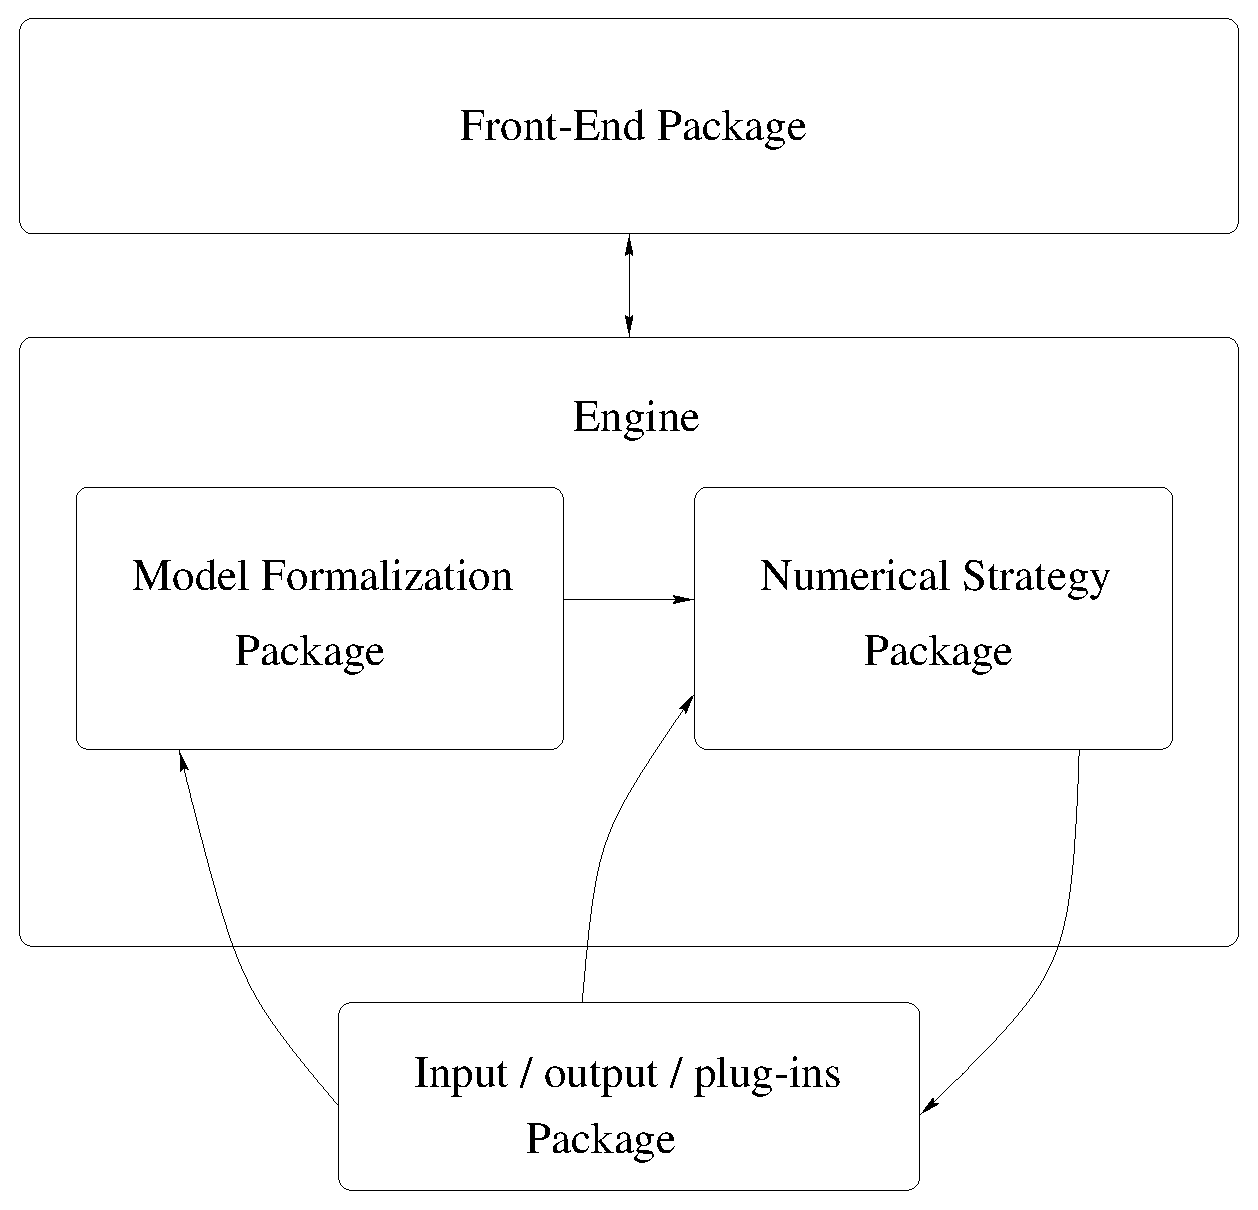
\includegraphics[scale=0.80]{figure/dependency.eps}
\caption{Structure chart of the dependencies}
\label{dependency}
\end{center}
\end{figure}

%\clearpage

The chart \ref{dependency} shows the links seen previously. The Front-end access the platform to drive a complete simulation. The model formalisation uses input methods (basic input method or input method form a dedicated plug-in) to get data, then other
methods to fill the data structure of the platform according to the specificities of each \ac{nsds}.
The numerical strategy uses the model built before to make the computations and an output method (basic output method or output method form a dedicated plug-in) to save the output data.\\

The following diagrams (\ref{sequence_diag1} \& \ref{sequence_diag2}) describe the unfolding of a simulation.
\begin{figure}[!hbp]
\begin{center}
\includegraphics[scale=0.65, bb=30 40 300 775,angle=-90, clip]{figure/sequence1.ps}
\caption{Sequence diagram - Without plug-in}
\label{sequence_diag1}
\end{center}
\end{figure}

\begin{figure}[!hbp]
\begin{center}
\includegraphics[scale=0.65, bb=30 40 330 775,angle=-90, clip]{figure/sequence2.ps}
\caption{Sequence diagram - With plug-in}
\label{sequence_diag2}
\end{center}
\end{figure}

\subsection{Interface view}
We will define in this section the functionalities of the components and their interfaces. 
% It should define the system using one or more of the identity, functions and interface parts of the component description. Suitable methods of presentation are interface files and parameter tables. The intended readership of this description comprises designers, programmers and testers, who need to know how to use the components in the system.
For each communication between components, the information in transit is detailed :
\begin{itemize}

        \item Front-End to Engine\\
        Input files name, matrices, systems, relations that the users want to use for the computations.

        \item Engine to Front-End\\
        Error messages, control messages (``Simulation finished'', indications about the current computation, \dots), some of the simulation result.
        
        \item Model Formalisation to Numerical Strategy\\
        Formalised model, which is composed of several equations (dynamical equation, relations and non smooth laws).
        Most of the equations are composed of matrix.
        
        \item Input/Output/Plug-ins to Model Formalisation\\
        Description of the physical problem. Reading of dedicated files by plug-ins or input/output methods.
        
        \item Plug-ins to Numerical Strategy\\
        Selection of the right methods for computations.
        
        \item Numerical Strategy to Input/Output/Plug-ins\\
        Description of the physical problem at the end or during the simulation.

\end{itemize}

\section{System architecture diagram with related description}
The figure \ref{archi} shows the system architecture using the SA method.
\begin{figure}[p]
\begin{center}
\includegraphics[angle=90, height=22cm]{figure/archi.pstex}
\caption{System architecture - SA diagram}
\label{archi}
\end{center}
\end{figure}
We can see in this figure, the different packages of the architecture.
At first, the package regrouping the input/output modules are represented in light blue and the plug-in modules are represented in dark blue.
In green we see the Front-end package.
In yellow, the Model formalisation package.
In pink, we see the numerical strategy.
Finally, the last module, "update state" is shared between the formalisation and the numerical
strategy package.\\

The diagram \ref{archi_sd} represents the structure we build with the SA diagram. This is the SD diagram.
The one who see is the restructured diagram.
\begin{figure}[p]
\begin{center}
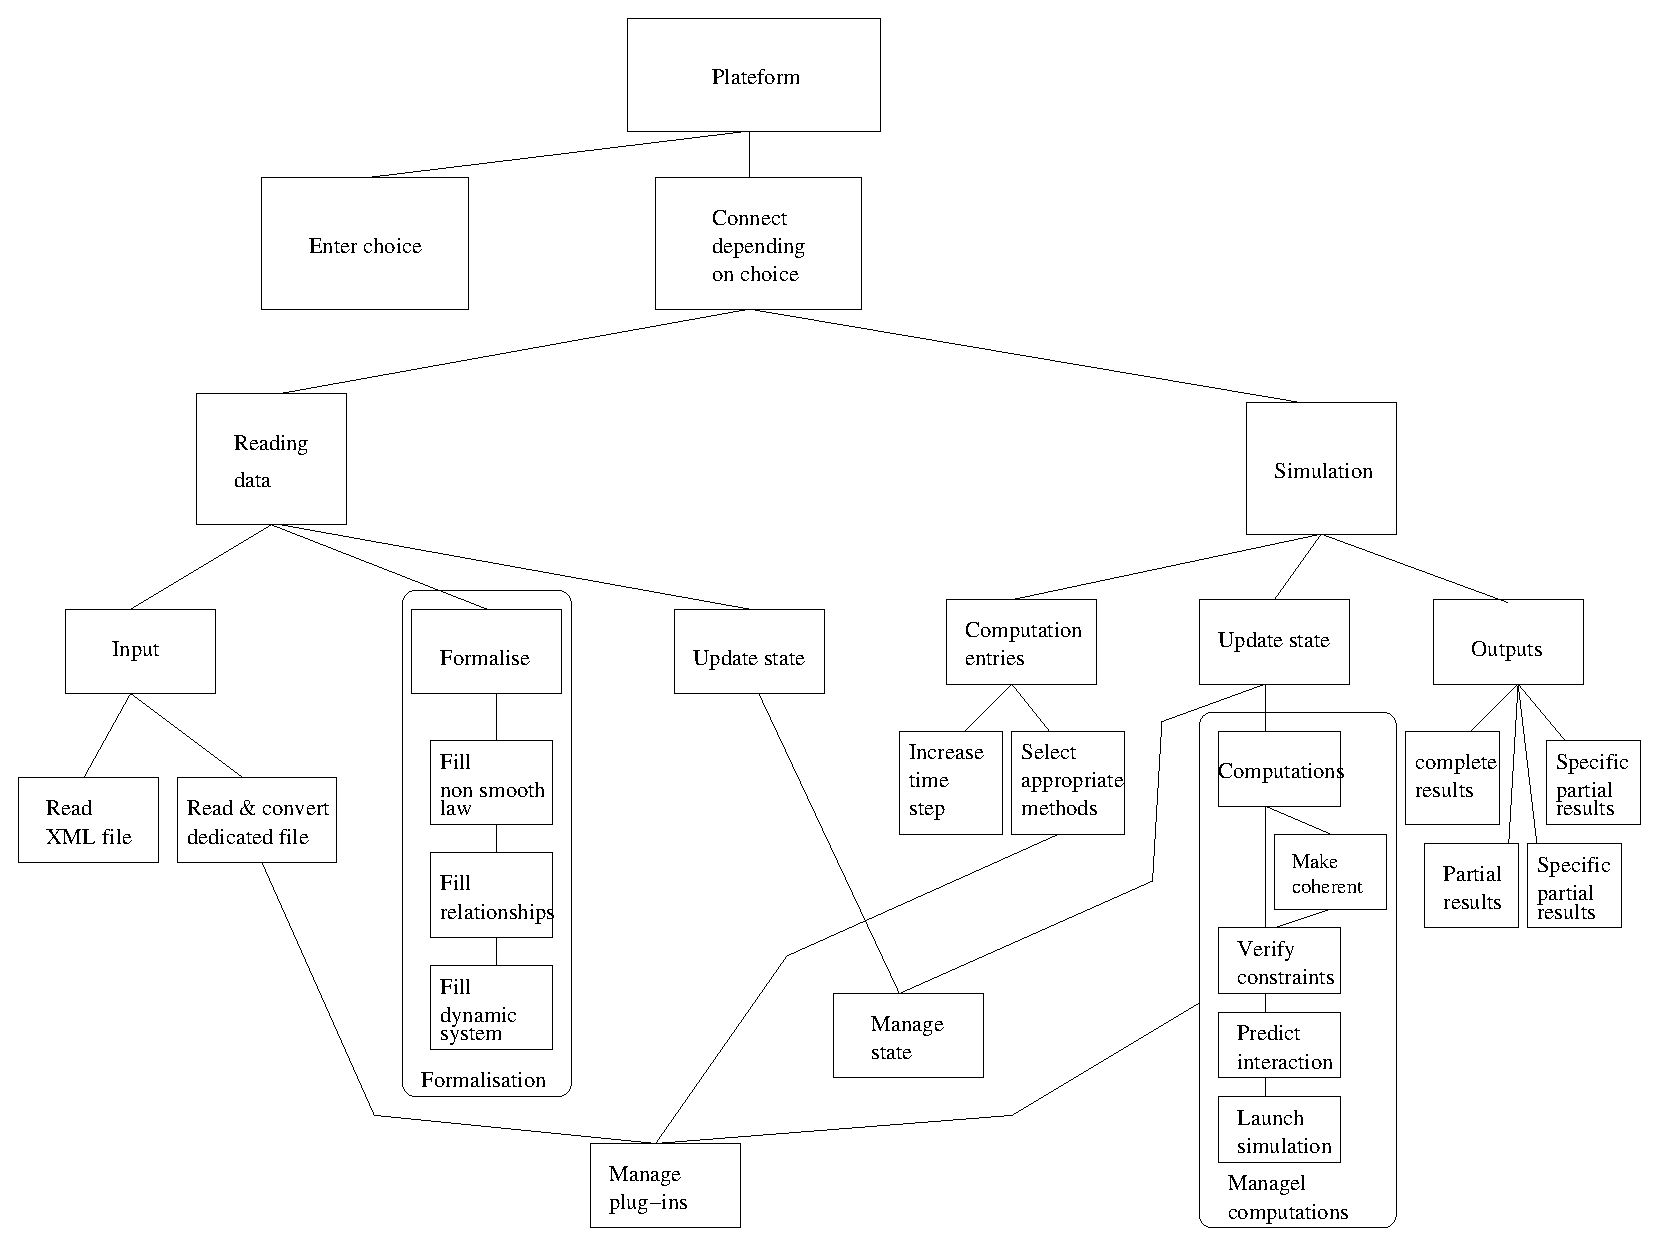
\includegraphics[angle=90, height=22cm]{figure/archi_sd.eps}
\caption{System architecture - SD diagram}
\label{archi_sd}
\end{center}
\end{figure}


\section{SASD conclusion}
The different groups we have made are high cohesion modules because they regroup specific traitments.
During the Detailed Design Phase, we must be carefull with the coupling between these modules.

%---------------------------------------------------------------------%
\newpage
\chapter{Component Description}
\label{Sec:SSD-ComponentDescription}
\section{\ac{lapack}}
It consists in routines for solving systems of simultaneous linear equations, least-squares solutions of linear systems of equations, eigenvalue problems, and singular value problems. The associated matrix factorizations (LU, Cholesky, QR, SVD, Schur, generalized Schur) are also provided, as are related computations such as reordering of the Schur factorizations and estimating condition numbers. Dense and banded matrices are handled, but not general sparse matrices. In all areas, similar functionality is provided for real and complex matrices, in both single and double precision.

\section{MP solver pack}
%\begin{ndr}
%	tell what we'll find in MP solver pack, the Primal Relay, DR, CFP, CFD, ...\\
%	put here some parts of the \ac{tm}
%\end{ndr}

For more details you can refer to the \ac{tm}.

\subsection{Definition of a \acs{lcp} problem}
Let $M$ be a given $n\times n$ matrix, and let $q$ be a given $n$ vector. The linear complementary problem is to find vectors $z$ and $w$ such that
\begin{eqnarray}
M z - w = q \label{equi}\\
z \ge 0, w \ge 0\label{comp}\\
z \cdot w = 0 \label{pdt}
\end{eqnarray}
%
Here, $(z_{i},w_{i})$ is a pair of complementary variables. A solution $(z,w)$ to the above system is called a complementary basic feasible solution if $(z,w)$ is a feasible%
\footnote{A numerical vector that satisfies all the constraints and restrictions in the problem is said a feasible solution.}
solution to $($\ref{equi}$)$ and $($\ref{comp}$)$ and if one variable of the pair $(z_{i},w_{i})$ is  basic% 
\footnote{Consider the following system of linear equality constraints 
\begin{eqnarray}
A x = b \label{basis} \\
x \geq 0
\end{eqnarray}
where $A$ is a given matrix of order $m\times n$ and $m$ is the rank of $A$.
A basis B for \ref{basis} is a square matrix consisting of $m$ columns of A which is nonsingular; and the column vector of variables $x_{B}$ associated with the columns in $B$, arranged in the same order, is the basic vector corresponding to it.
} 
for $i=1,..,n.$




\subsection{Definition of a \acs{cp} problem}
The aim of generalized Non--smooth Newton methods is to provide numerical solutions of systems of nonsmooth equations of the form :
\begin{eqnarray}
  \label{eq:1}
  H(x)=0
\end{eqnarray}
where $H:\Omega \subset \RR^n \mapsto \RR^n $ is locally Lipschitz on the open set $\Omega$. 

If the function $H$ is differentiable on $\Omega$, classical Newton  methods and its variants may be used to solve the equation \eqref{eq:1} and several theorem of local convergence may be formulated. The non differentiability of $H$ gives rise to a lot of complications that invalidates the classical methods.




\subsection{Definition of a Relay problem}
The relay system can be written as a LCP by introducing extra variables. It is convenient to express a standard LCP using the convex analysis formalism:
$$0\le z \perp w \ge 0 \iff -w \in \partial\psi_{[0,+\infty[}(z)$$
Consequently a relay system is synthetically written as follows:
\begin{eqnarray}
Mz-w=q\label{relequi}\\
-w \in \partial\psi_{[-s,s]}(z)\label{relcomp} 
\end{eqnarray}

By extension the set $[-s,s]$ is considered for vector valued problems as the cartesian product of intervals,\\
$$ [-s,s]=\prod_{i=1}^{n}[-s_{i},s_{i}]$$
Set $w^+$ and $w^-$ the positive part and the negative part of $w$, $w=w^+-w^-$ with $w^+=max(w,0)$, $w^-=max(-w,0)$. We introduce two extra variables defined as follows:\\
$z^{p}=s+z ; z^{m}=s-z $ such that $z^{p}+z^{m}=2s$\\


\subsection{Solving routines}
MP solver pack provides solvers for the previous problems. In the one hand, the basics \ac{lcp} solvers for \ac{lcp} problems, and in the other hand extended solvers for \ac{pr}, \ac{dr}, \ac{cfp}, \ac{cfd} problems.



\section{\ac{ode} pack}
It consists of nine solvers, namely a basic solver called LSODE and eight variants of it -- LSODES, LSODA, LSODAR, LSODPK, LSODKR, LSODI, LSOIBT, and LSODIS. The collection is suitable for both stiff and nonstiff systems.  It includes solvers for systems given in explicit form, dy/dt = f(t,y), and also solvers for systems given in linearly implicit form,  A(t,y) dy/dt = g(t,y).  Two of the solvers use general sparse matrix solvers for the linear systems that arise.  Two others use iterative (preconditioned Krylov) methods instead of direct methods for these linear systems.  The most recent addition is LSODIS, which solves implicit problems with general sparse treatment of all matrices involved.



%---------------------------------------------------------------------%
\newpage
\printglosstex(acr)[p]

%===================================

\listoffigures
\listoftables
\cleardoublepage
%\bibliographystyle{plainnat}
%\bibliography{./Biblio/String,./Biblio/Cp.bib,./Biblio/Optim.bib,./Biblio/Contact.bib,./Biblio/NonSmooth.bib,./Biblio/Leger.bib,./Biblio/Petri.bib}
\cleardoublepage
\end{document}
